%aum ganathipathaye namaha
%sri rama jeyam

%aum ganathipathaye namaha
%sri rama jeyam
\section{Background and Problem Statement} \label{sec:prob_state}
%Identifying semantically similar or equivalent binary code is a challenging task.
%In this section, %we discuss the problems of the existing binary code search techniques with motivating examples.
%Then
In this section, we provide a motivating example that emphasize on the need for true semantics analysis of functions and necessity to have a function model that is agnostic to underlying program structure. Later, explain the key challenges 
%(\textbf{P1-3}) 
faced by existing binary function matching tools in detail. Finally, we explain the basic idea of our proposed solution.

%we \xyx{give a motivating example of binary matching regardless of architecture and OS differences, and state the challenges of  binary code search in finding the semantics and structures for this example. Last, we explain the basic idea of our proposed solution. }%and discuss their roles to achieve the scalable binary matching regardless of architecture and OS differences.}

\subsection{Motivating Example}  \label{subsec:bin_pre}

A binary program consists of a set of functions, where each function is a (directed) graph of basic-blocks, i.e., CFG (control-flow graph). The instructions in a function are systematically  grouped into several basic-blocks, which are considered as the building blocks of binary program and this representation is used by many static binary analysis tools.
%\begin{mydef}
%\emph{(\textbf{Basic-block}) A sequence of assembly instructions without any jumps or jump targets in the middle, where a jump target starts a block, and a jump ends a block.}
%\end{mydef}
\begin{figure}[ht]
  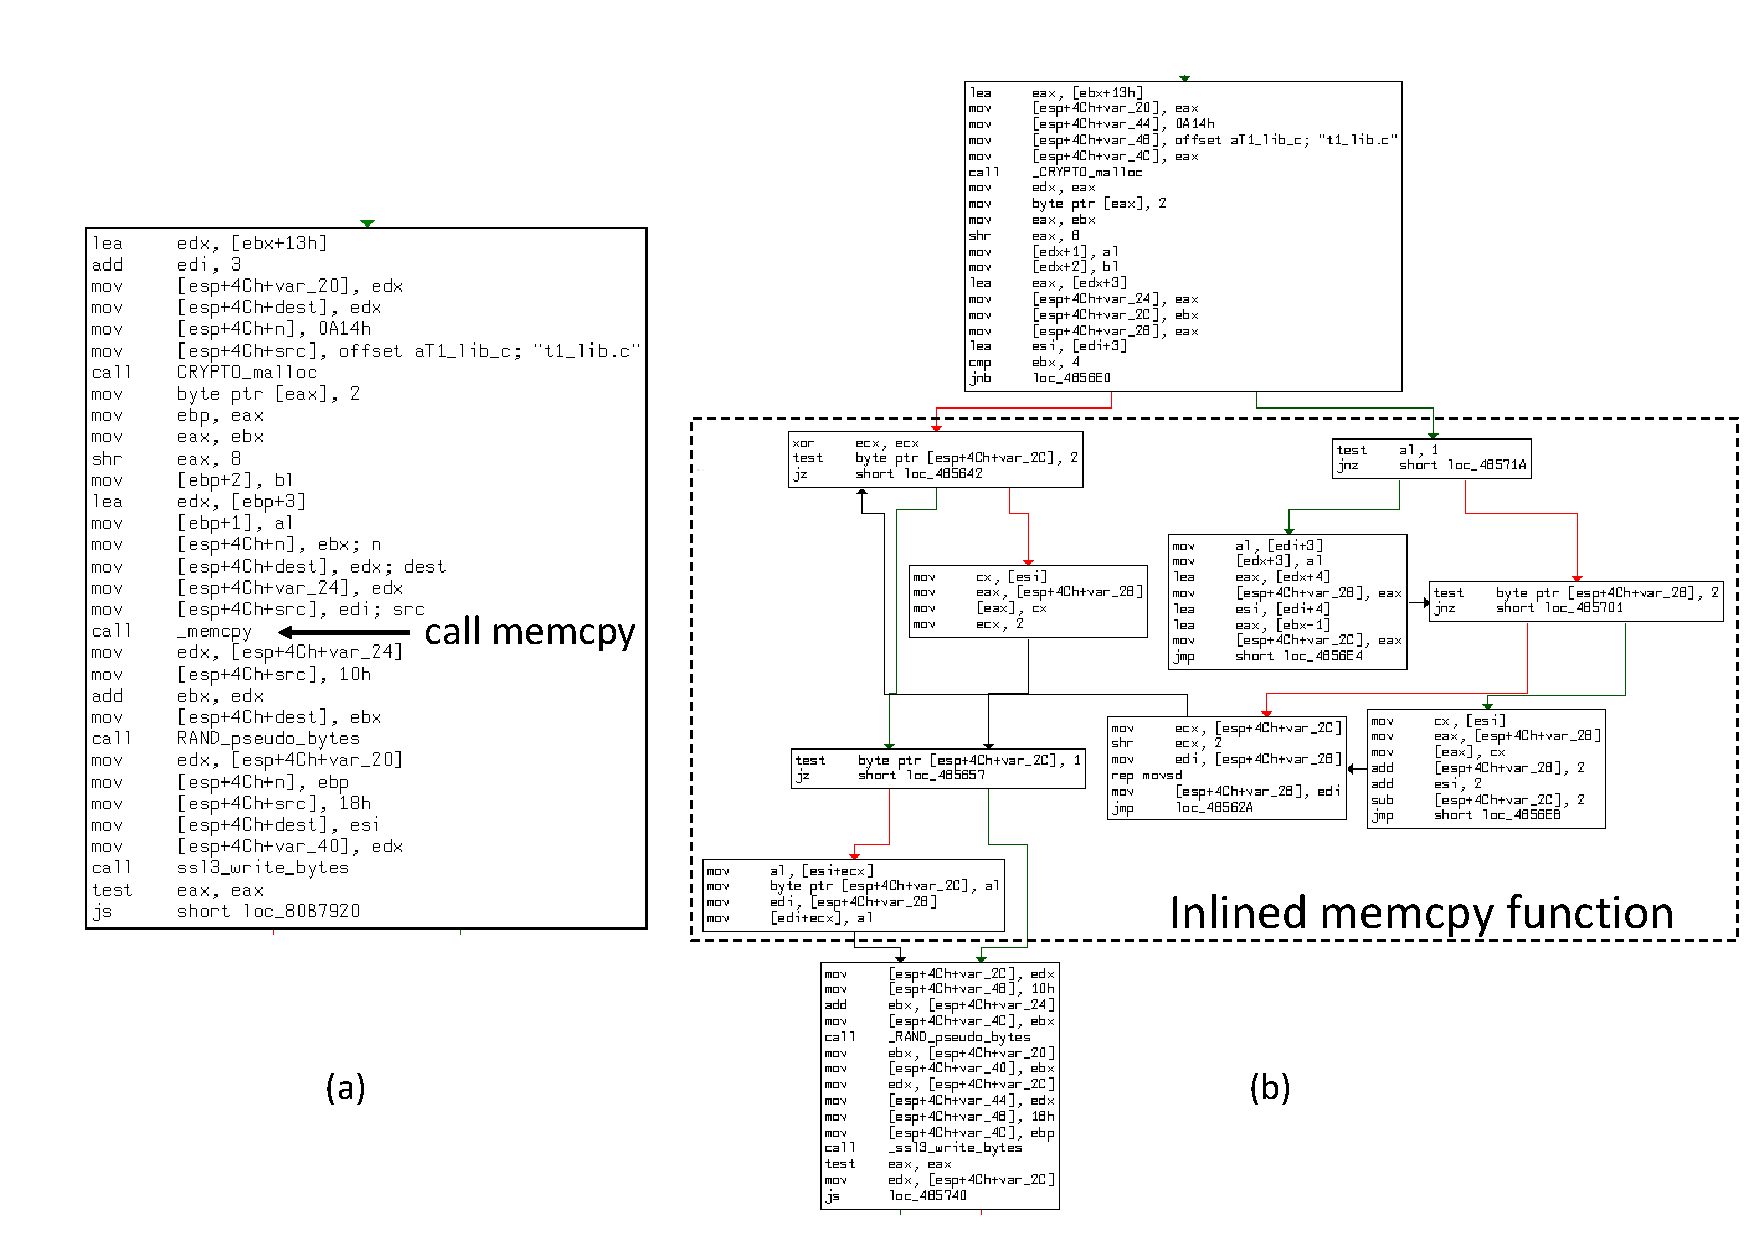
\includegraphics[width=\linewidth]{srj-figures/srj-moti_ex2.pdf}
  \caption{Code segment responsible for Heartbleed vulnerability (CVE-2014-0160) appeared as in the binary (a) compiled with GCC 4.6, and (b) compiled with Mingw32} \label{fig:prob_stat}
\end{figure}

%\begin{example}
Interestingly, the same source code may have different basic block structures after compilation. For example, Fig.~\ref{fig:prob_stat} shows the code segment responsible for the infamous heartbleed vulnerability (CVE-2014-0160), where Fig.~\ref{fig:prob_stat}(b) and (c) show the basic block structure when compiled the source code with \texttt{gcc} and \texttt{mingw}, respectively. Apparently, these two binary code segments share no identical basic-block structures --- with \texttt{gcc}, the vulnerable code is represented as a single basic block;  with \texttt{mingw}, represented as several basic blocks. A deeper inspection suggests that in \texttt{mingw} version the library function \texttt{memcpy} is inlined; while in \texttt{gcc}, it is not. %Due to this library function inlining, in \texttt{mingw}, the similarity between basic-blocks is affected considerably.
Given the \texttt{gcc} version as a signature, we may miss the vulnerability in \texttt{mingw} version due to function inlining. 

Hence, basic-block centric  
%function modeling
similarity matching(\textbf{P1}) and \mahin{program structure dependent pre-fitlering (\textbf{P3})} is not robust enough to address real-world problems. Further, this real-world scenario strongly suggest that functions should not be analysed in isolation, i.e., to capture the true semantics of a functions (\textit{caller}), all the related functions (\textit{callee}) also need to be taken in to consideration based on the caller-callee relationship (\textbf{P2}).
%\end{example}

 % and it is formally defined as follows (adapted from~\cite{david2014tracelet}):
%
%\begin{mydef}
%\emph{(\textbf{Type-k Partial Trace\footnote{In the rest of the sections, we'll use the term `partial trace' and `type-k partial trace' interchangeably, where `type-k partial trace' is used when referring to the length of a partial trace and in all other instances the term `partial trace` is used}}) Type-k partial traces is an ordered tuple of $k$ sequences, each representing one of the basic-blocks in a directed acyclic sub-path in the CFG, and containing all of the basic-block's assembly instructions.
%}
%\end{mydef}


%We introduce the term \emph{environment}, where binary is generated and executed, to denote the underlining architecture (e.g., Intel, ARM), the operating systems (OS) (e.g., Windows, Linux), the used compiler, and also the chosen compilation options.
%Different architectures have different instructions (a.k.a. ISA or Instruction Set Architecture) for the machine.
%Obviously, different environments will lead to considerably different binaries.

%\note{\textbf{I think we need make sure environment is used in the rest of the sections}}


%To better find the assembly code clones that perform similarly computational tasks, we formulate the concept of semantic clones.

% which has very important applications in both software security and software engineering. Despite the challenges, in the recent year, there are several good solutions proposed in academia to tackle this problem~\cite{pewnycross,ruttenberg2014identifying,egele2014blanket,luo2014semantics}. %of identifying semantically equivalent functions at binary level.
%However, none of the existing studies fills up the theory blank of \lq{}how a function is modelled\rq. %In the proposed modelling techniques of {\color{red}{using XXX}}~\cite{pewnycross,luo2014semantics}, it is assumed that basic-block structure is preserved across binaries, and thus, functions models should be  basic-block centric. Based on this assumption, semantic features are extracted from the sample functions at basic-block level and compared with the counterparts extracted from target functions in a pairwise way of basic-block comparison.


\subsection{Challenges for Syntax-based Matching}

%\textcolor{red}{//the state-of-the-art binary search}

%\textcolor{red}{//a motivating example}

%\textcolor{red}{//modeling the binary code}
%
%\begin{figure*}[ht]
% \begin{minipage}{.3\textwidth}
%\lstinputlisting[language=C]{srj-figures/srj-openssl_code.c}
%   (a)
%\end{minipage}
% \begin{minipage}{.3\textwidth}
%  \centering
%     (b)
%  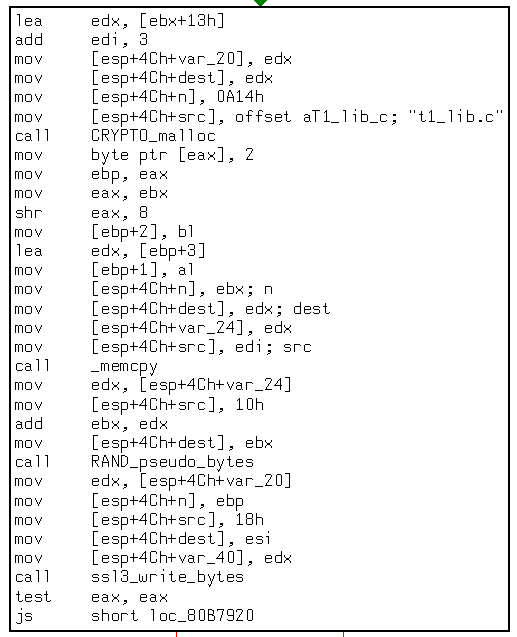
\includegraphics[height=4cm]{srj-figures/srj-gcc.png}
%  \end{minipage}
%  \begin{minipage}{.3\textwidth}
%
%   \centering
%  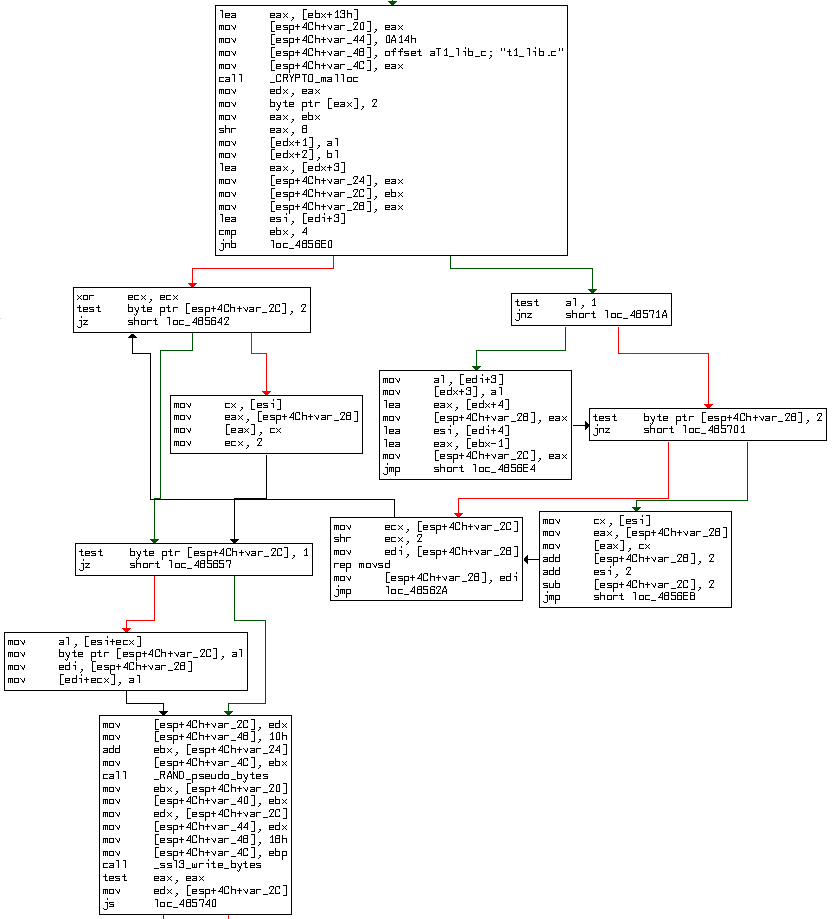
\includegraphics[height=6cm]{srj-figures/srj-mingw32.png}
%     (c)
%   \end{minipage}
%  \caption{SSL/Heartbleed vulnerability (CVE-2014-0160) appeared as in the (a) actual source code, (b) binary compiled with GCC 4.6 for Linux OS, and (c) binary compiled with Mingw32 for Windows OS} \label{fig:prob_stat}
%\end{figure*}

Syntax is the most direct information that can be used for matching. 
\xyx{Existing approaches mostly have attempted to use instruction patterns, e.g., $n$-gram~\cite{DBLP:conf/uss/JangWB13}, graphlet~\cite{DBLP:conf/raid/KrugelKMRV05} and tracelet~\cite{DBLP:conf/pldi/DavidY14} patterns of instructions in the basic blocks, to match binaries. For matching accuracy, these approaches rely on syntax information (e.g., instruction type) for matching.}
However, \xyx{relying on instruction syntax assumes that the systems are running in the same environment, \emph{i.e., the same architecture, same OS, and compiled with same compiler and compiler options}}.
%These techniques rely on the syntactic characteristics of functions~\cite{DBLP:conf/pldi/DavidY14,jang2011bitshred}, by which the function similarity is measured at the binary syntax level.
Though these techniques work well for the given environment (e.g., cases presented in~\cite{DBLP:conf/pldi/DavidY14}), it  fails for cross-architecture and cross-OS analysis, \xyx{where syntax dramatically changes for the different enviroments that it runs on~\cite{DBLP:conf/sp/PewnyGGRH15}}.

Clearly, the key challenge for syntax-based matching is:
\noindent \textbf{C1: There is no consistent binary syntax representation in different environments.}
For example, the two binary code segments in Fig. \ref{fig:idiom2-ex}, one for ARM and one for x86 32bit,  both represent the behaviours of stack frame setup in function prologue. However, by relying on \xyx{the direct} syntax representation, it is hard to match them.


\subsection{Challenges for Semantics-based Matching} \label{subsec:sem_chall}

To make the matching tolerant to the syntax difference in binaries, semantics-based matching has been proposed~\cite{luo2014semantics,DBLP:conf/sp/PewnyGGRH15}, which use the machine state transition to represent the semantics of the binary. However, there are three challenges in adopting the semantic information in binary matching.

\textbf{C2: How to choose the segments of binary for the semantics calculation.}
Existing approaches~\cite{luo2014semantics,DBLP:conf/sp/PewnyGGRH15} assume that basic-block structure is preserved across binaries, thus the matching should be basic-block centric. Based on this, models or features extracted from the given binary segment at basic-block level are compared with the counterparts extracted from target functions in a pairwise way. In practise, the strong assumptions behind are too restrictive to be applied for real-world cases. The following quote from~\cite{DBLP:conf/sp/PewnyGGRH15} clearly sums up the problem in such assumption:
\emph{"Our metric is sensitive to the CFG and the segmentation of the basic block, which we found to be potentially problematic especially for smaller functions."}

\note{\noindent\textbf{%how existing techniques fail to capture \textit{true semantics} of the function, only partial semantics are captured. 
C3. How much contextual semantics is needed to complement the basic-block centric (syntactic and structural) matching.}}
\xyx{Some existing techniques~\cite{wang2015binary} has noticed	the problem of basic-block, and propose to \textit{blindly} inline all the user-define functions (non-inline the library functions). %The blindly inlining strategy would lead to such a problem of code size explosion that the bloated functions are hard to analyze, incurring heavy overhead. 
%However, one might assume that inlining all the callee functions at their respective call sites, as in~\cite{wang2015binary}, would solve the partial (or incomplete) semantics problem present in existing binary function matching techniques.
Unfortunately, this approach do not work in practise due to two main reasons: (1) heavy inlining may lead to code size explosion~\cite{chang1992profile}, where performing similarity matching on bloated functions incur heavy overhead and hence, not scalable to real-world binary analysis, and (2) not all the callee functions (both user-defined and library functions) are closely related, in-terms of functionality, to the caller function, hence, inlining such functions might dilute the core functionality of the caller function, which in return, leads to poor matching results.} \note{\textbf{??Mahin, can you give an example or some citation.}}


%
%\noindent\textbf{C2: Semantics of binary code is too low level.}
%Due to the lack of explicit program semantics at binary level, machine state transitions of two totally unrelated code segments may look very similar (or identical), if the number of instructions in those binary segments are too small, e.g., the two code segments in Fig.~\ref{fig:code_seg}.
%A binary modeling approach based on machine state transitions has the problem of producing high false positives, especially when the given function (or vulnerability) signature is too small~\cite{DBLP:conf/sp/PewnyGGRH15}.
%%\ly{combine fig 2 and 3?}
%%Unfortunately, signatures, especially vulnerability signatures, having few instructions is common in real-world scenarios~
%
%\begin{figure}[t]
%\scriptsize
%  \begin{subfigure}[b]{0.4\linewidth}
%  \begin{equation}
%  \boxed{
%\begin{aligned}
% \mathtt{ADD \quad EAX,EBX}
%\end{aligned}}
%\end{equation}
%   \label{fig:seg1}
%  \end{subfigure}%%
%  \begin{subfigure}[b]{0.4\linewidth}
%   \begin{equation}
%   \boxed{
%\begin{aligned}
% &\mathtt{PUSH \quad EBX} \\
% &\mathtt{CALL \quad strlen} \\
% &\mathtt{CMP \quad EAX,0}
%\end{aligned}}
%\end{equation}
%    \label{fig:seg2}
%  \end{subfigure}%%
%  \vspace{-3mm}
%  \caption{Sample code segments}
%  \label{fig:code_seg}
%\end{figure}
%
%As shown in Fig. \ref{fig:state_seg}, two unrelated segments in Fig.~\ref{fig:code_seg} have the same initial machine state (i.e., pre-state) and also the identical post-state after execution. %, both code segments will result in .
%Here, code segment 1 adds the values in $\mathtt{EAX}$ and $\mathtt{EBX}$ registers, and move the results to $\mathtt{EAX}$ register. Since the pre-state values are all set to zero, after execution, $\mathtt{EAX}$ register will hold the value 0 and the condition-code flag $\mathtt{ZF}$ (zero flag) will be set to 1, since the result of addition operation is zero. On the other hand, in code segment 2, the value in $\mathtt{EBX}$ register is pushed to the stack, system API $\mathtt{strlen}$ is invoked, and finally the return value that is stored in $\mathtt{EAX}$ register is compared with an immediate value `0'. After execution, similar to code segment 1, $\mathtt{EAX}$ register will hold the value 1 as $\mathtt{strlen}$ system API is not interpreted (e.g., \cite{DBLP:conf/sp/PewnyGGRH15,luo2014semantics}), $\mathtt{EAX}$ register will hold the pre-state value, which is 0. In addition, the comparison operation will set the $\mathtt{ZF}$ to 1. In both executions, none of the other registers, condition-code flags and memory locations will be modified, hence retaining the pre-state values. From the examples shown in Fig.~\ref{fig:code_seg} and~\ref{fig:state_seg}, it can be seen that machine state transitions alone are not sufficient to model binary code.
%%\end{example}

%\noindent \textbf{C3: Computing the precise semantics is difficult and expensive.}
%Static methods~\cite{luo2014semantics,DBLP:conf/sp/PewnyGGRH15} using state-based semantic computation cannot capture the precise semantics due to missing the consideration of system APIs in the analysis.
%Dynamic analysis based techniques such as~\cite{egele2014blanket} might be able to address this problem. However, it is not scalable enough to handle large binaries. For example, in \cite{egele2014blanket}, before each function is executed, an environment needs to be set so that the execution does not terminate due to uninitialised memory handling. Unfortunately, considering the fact that a moderate size binary would easily have several thousand functions, this approach is not very scalable. %Hence, to address these challenges, we propose a partial traces based function modelling technique.



%\begin{figure}[t]
%\small
%  \begin{subfigure}[b]{0.45\linewidth}
%  \begin{equation*}
%\begin{aligned}
%    &\text{\textbf{Pre-state:}}\\
%    &\mathtt{Reg = \lbrace EAX=0, EBX=0 \ldots \rbrace} \\
%    & \mathtt{Flag = \lbrace ZF=0, PF=0 \ldots \rbrace} \\
%    & \mathtt{Mem=\lbrace 0,0 \ldots 0 \rbrace}
%    \end{aligned}
%\end{equation*}
% \begin{equation*}
%\begin{aligned}
%    &\text{\textbf{Post-state:}}\\
%    &\mathtt{Reg = \lbrace EAX^\prime=0, EBX=0 \ldots \rbrace} \\
%    & \mathtt{Flag = \lbrace ZF^\prime=1, PF=0 \ldots \rbrace} \\
%    & \mathtt{Mem=\lbrace 0,0 \ldots 0 \rbrace}
%    \end{aligned}
%\end{equation*}
%    \label{fig:state_seg1}
%       \caption{state transitions for Fig.~\ref{fig:code_seg}(1)}
%  \end{subfigure}
%  \begin{subfigure}[b]{0.5\linewidth}
%    \begin{equation*}
%\begin{aligned}
%    &\text{\textbf{Pre-state:}}\\
%    &\mathtt{Reg = \lbrace EAX=0, EBX=0 \ldots \rbrace} \\
%    & \mathtt{Flag = \lbrace ZF=0, PF=0 \ldots \rbrace} \\
%    & \mathtt{Mem=\lbrace 0,0 \ldots 0 \rbrace}
%    \end{aligned}
%\end{equation*}
% \begin{equation*}
%\begin{aligned}
%    &\text{\textbf{Post-state:}}\\
%    &\mathtt{Reg = \lbrace EAX^\prime=0, EBX=0 \ldots \rbrace} \\
%    & \mathtt{Flag = \lbrace ZF^\prime=1, PF=0 \ldots \rbrace} \\
%    & \mathtt{Mem=\lbrace 0,0 \ldots 0 \rbrace}
%    \end{aligned}
%\end{equation*}
%    \label{fig:state_seg1}
%    \caption{state transitions for Fig.~\ref{fig:code_seg}(2)}
%  \end{subfigure}
%  \caption{Machine state transitions for code segments in Fig.~\ref{fig:code_seg}}
%  \label{fig:state_seg}
%\end{figure}





\subsection{Proposed Solution} \label{subsec:motivate_eg}


\xyx{To overcome C1, we propose to convert the instructions into the IR for cross-architecture and cross-OS analysis. To   mitigate C2, we borrow the idea of tracelet used in \textsc{\small Tracy}~\cite{DBLP:conf/pldi/DavidY14}. Different from the fixed length of 3-tracelet, we use a variant length of partial traces to mitigate the affect of basic-block granularity. Last, to address C3, we propose a selective strategy to strike a balance between the needed contextual semantic and the overheads due to inlining. }

 

\begin{mydef} \label{def:tracelet}
\emph{\textbf{A partial trace} is \note{an instruction sequence obtained from basic-blocks that lie adjacent to each other along a program execution path. Partial traces can be of different length, where partial trace of length $k$ (called, Length-$k$ partial trace) denotes a partial trace that contains the instructions obtained from $k$ adjacent basic-blocks that lie along a program execution pat }}
\end{mydef}

\begin{mydef} \label{def:comp_semantic}
\emph{\xyx{\textbf{Complete (or true) Semantics} refer to the contextual semantics that the function under analysis and %why we need true semantics of a function because compiler inline/outline certain functions
}}
\end{mydef}


%As discussed in Section \ref{sec:prob_state}, 
The existing static binary function matching techniques, in general, fail to take into account the true (or complete) semantics of the functions under investigation. That is, each function in a binary is analyzed in isolation, where the semantics of the callee functions (be it user-defined or library function) are not considered when generating the caller function semantics as they are assumed to be two different functions. However, this assumption is intuitive and valid until we understand the caller-callee relationship (or dependency). For example, assume a user-defined function that manipulates string literals invokes the \texttt{strcpy} library function, and in order to capture the true semantics of the caller, it is \note{essential?} to inline \texttt{strcpy} function at the call site, as the caller function is involved in string manipulation, where it leverages on utility fucntions, such as \texttt{strcpy}, provided by the C runtime library to simplyfy its operations, hence, the semantics of the utility functions need to be considered as part of the caller fucntion semantics. Similarly, in another occasion, the programmer might implement her own version of \texttt{strcpy} function with additional security properties (called, \texttt{strcpy\_secure}\footnote{It is worth noting that \texttt{strcpy} is one of the banned function calls by Microsoft and hence, its better to use more secure variants such as \texttt{strncpy\_s} and \texttt{strcpy\_s}~\cite{msbannedfunctioncalls}}) and invokes it from all the string manipulation functions that need a secure string copy operation, hence, to capture the true caller semantics, the user-defined \texttt{strcpy\_secure} function needs to be inlined at the call site.

%To this end, in this paper, we propose partial trace based function modelling to overcome the aforementioned limitation.

%\noindent\textbf{$3$-tracelet or $k$-tracelet?}  In \cite{DBLP:conf/pldi/DavidY14}, $3$-tracelet, a concatenation of 3 adjacent basic-blocks, is used for searching. \textcolor{red}{Why k-tracelet is better.}


%Semantic based vulnerability detection at binary code level is an active research area and a promising direction towards securing closed-source software programs. However, we find that there is a gap in existing work \cite{pewnycross}\cite{ruttenberg2014identifying}, especially in vulnerability modelling, that is worth exploring. In the proposed vulnerability modelling techniques, it is assumed that basic-block structure is preserved across binaries \cite{pewnycross}, and thus, vulnerabilities are modelled basic-block centric. That is, semantic features are extract for from the basic-blocks in the known vulnerable function and they are compared with the basic-blocks in the target functions to identify the staring points of potential vulnerabilities.

%In \cite{ruttenberg2014identifying}, it is reported that for each basic-block in the signature (called, \textit{starting points}), first 20 basic-blocks (in-terms of similarity), in the target program, are selected for further signature matching. Similarly, in \cite{pewnycross}, for each basic-block in the signature, first 200 candidate basic-blocks, in the target program, are selected for the next level of vulnerability signature matching, using a greedy BHB (Best-Hit Boarding) algorithm. The commonality between these approaches is that the starting points, for vulnerability signature matching, are selected based on the similarity between basic-blocks in signature and target programs. However, the major drawback in this approach is that the basic-block structures can be easily distorted by factors that are beyond the control of security analysts.

%For example, figure \ref{fig:prob_stat}(a) shows the well-known heartbleed vulnerability (CVE-2014-0160) that shook the entire software industry. Figure \ref{fig:prob_stat}(a) shows the vulnerability at binary code level, compiled with GCC-4.6 and (c) shows the same vulnerability, but compiled with MinGW32. Immediately, we can say that the two programs doesn't share same basic-block structure. That is, with GCC, the vulnerable code is represented as a single basic-block, however, with MinGW, it is split into several basic-blocks. A deeper inspection would suggest that in MinGW version the library function \texttt{memcpy} is inlined while in GCC, it is not. Due to this library function inlining, in MinGW, the similarity between basic-blocks is affected considerably. That is, given the GCC version as a signature, we may miss the vulnerability in MinGW version due to basic-block \textit{splitting} and \textit{vice-versa} due to basic-block \textit{merging}. Hence, basic-block centric vulnerably modelling may not be robust against factors such as compiler type (version), optimization level and even difference in build environments. Therefore, in this paper, we present a more robust, self-adoptable vulnerability modelling technique.

%\todo {\color{blue} Do I need to include scope here? like doesn't not consider obfuscated binary that are hard to disassemble and only consider clean binaries without any obfuscations/packing.}

%\subsection{Problem Statement and Possible Solution} \label{subsec:pos_sol}
%To compare binaries, we need to define the criteria to compute similarity.
%In this work, we propose two complementary criteria to capture the semantic and structural information of the binary programs.
%Let $\mathcal{I}_1$ and $\mathcal{I}_2$ be two partial traces, we formally define the two kinds of similarity as follows:
%%The function $\langle\!\langle inst \rangle\!\rangle$ converts an instruction sequence (or an instruction) into a corresponding symbolic expression.
%
%
%\begin{mydef} \label{def:sem_sim}
%\emph{(\textbf{Semantic Similarity})
%Let $s_0$ denote a pre-state before executing $\mathcal{I}$, and $s_1=\langle\!\langle s_0, \mathcal{I}\rangle\!\rangle$ denote post-state after executing $\mathcal{I}$ on $s_0$. %post_\mathcal{I}^{pre_{\mathcal{I}}}=
%Let $S$ be set of all possible pre-states values that both $\mathcal{I}_1$ and $\mathcal{I}_2$ can execute on.
%The semantic similarity of $\mathcal{I}_1$ and $\mathcal{I}_2$, $SemSim(\mathcal{I}_1, \mathcal{I}_2)$, is defined as
%$\sum\nolimits_{s \in S} (\langle\!\langle s, \mathcal{I}_1\rangle\!\rangle -_m \langle\!\langle s, \mathcal{I}_2\rangle\!\rangle)$, where $-_m$ is a function to measure the difference of two machine states.
%%, the function $\langle\!\langle \bullet \rangle\!\rangle$ converts a partial trace into a set of \emph{symbolic expressions} and $\langle\!\langle \mathcal{I} \rangle\!\rangle(s)$ denotes assigning pre-state values $s$ to the symbolic expressions to yield the post-state values $ \mathcal{I}(s)$
%% are so \emph{similar in IO semantics} that they perform the similar computation tasks, if $PreS(\mathcal{I}_1)\approx reS(\mathcal{I}_2)$ and $PostS(\mathcal{I}_1)\approx PostS(\mathcal{I}_2)$.
%}
%\end{mydef}
%
%
%%In this work, a machine state is defined by the values stored at registers, condition-code flags and memory locations, which are common in all computing architectures.
%Semantic similarity is defined to capture the difference of the effects (i.e., post-state) of the binary program execution from the same input.
%Note that to calculate the precise effects of the program, we also need to consider the OS relevant information, like system API.
%Therefore, we consider that semantic similarity is architecture independent and OS dependent.
%
%%\ly{give one example of two code seg with different syntax, but same semantics}
%%Like example two in Fig. \ref{fig:state_seg}, the two code segments are not necessary to be from the same architecture, as the state model is not based on information that is architecture specific (see Section XX).
%
%Semantic similarity is one essential criteria to capture the behavior similarity of programs.
%However, this definition ignores the difference of program's structures, i.e., the program is treated as a black box.
%Due to the challenge \textbf{C2}, when comparing two binaries, we also want to consider the structures of the binary to make sure they are implementing the same algorithm or computation.
%%For example, bubble sort should not match with quick sort although they are semantically identical.
%This is critical in the tasks like code auditing, plagiarism detection and vulnerability detection.
%
%\begin{mydef} \label{def:comp_sim}
%\emph{(\textbf{Structural Similarity})
%The structural similarity of $\mathcal{I}_1$ and $\mathcal{I}_2$, $StrSim(\mathcal{I}_1, \mathcal{I}_2)$, is defined as
%$f^p_a(\mathcal{I}_1) -_f f^{p'}_{a'}(\mathcal{I}_2)$, where  $f^{p}_a(\mathcal{I}_1)$ (or $f^{p'}_{a'}(\mathcal{I}_2)$) is an abstraction function that maps $\mathcal{I}_1$ (or $\mathcal{I}_2$) to a structural model on architecture $a$, OS $p$ (or on architecture $a'$, OS $p'$); and $-_s$ is a function to measure the difference of two structural models.
%}
%\end{mydef}
%
%
%Structural similarity is a general definition. %, which aims to capture the high-level behavior of the binary code.
%The actual design of the abstraction function $f$ (e.g., using instruction patterns: $n$-gram~\cite{DBLP:conf/uss/JangWB13}, graphlet~\cite{DBLP:conf/raid/KrugelKMRV05} and tracelet~\cite{DBLP:conf/pldi/DavidY14}) reflects different research approaches on how to abstract the structural information of the binaries.
%Other usable structural information includes AST, PDG, data flow, type information and loop information.
%%For example, AST and PDG have been widely used for clone detection which reflect the syntax similarity.
%It is clear that the abstraction function is usually architecture and OS dependent, e.g., the codes in Fig.~\ref{fig:idiom2-ex}.
%%(e.g., using AST, PDG, data flow, type information, API and loop information)
%%Since the structureal information of assembly code (e.g., CFG) is usually architecture and OS specific, the direct matching based on CFG is not accurate, as shown in Fig. \ref{fig:prob_stat}. In this paper, we consider program information beyond the syntactic structure of the assembly code --- in addition, we also consider  data flow, type, API and loop information.
%
%%To capture the information relevant to semantics, we mainly consider data flow, API and partial traces in our model, while the structural information like BB is not the focus of our model.
%
%
%Overall, the similarity of $\mathcal{I}_1$ and $\mathcal{I}_2$ is defined as the combination of their semantic similarity and structural similarity.
%This similarity definition naturally resolves the challenge \textbf{C2}.
%
%To solve \textbf{C1}, we need to define a structural model, which is robust to different architectures and OSs. Motivated by the recent work on source code level idiom mining~\cite{allamanis2014mining},
%we propose to use the common binary patterns in different architectures and OSs as idioms, and use idioms to capture the program structural information, i.e., to define the abstraction function $f$.
%To support cross environments analysis, we propose a mapping of idioms in different architectures and OSs to a common concept such that $-_s$ can be easily computed.
%
%To solve \textbf{C3}, we propose a static analysis to capture the state-based semantics~\cite{DBLP:conf/sp/PewnyGGRH15} so that our approach is scalable.
%To capture the missing semantics related to system API using the static analysis, we introduce API idioms to complete the semantic information.
%Although the semantic comparison in this way is not precise as dynamic analysis like~\cite{egele2014blanket}, it works well with good scalability as shown in experiments.
%Furthermore, the idiom approach addresses the OS dependency problem in the semantic similarity definition.
%
%To solve \textbf{C4}, we propose a partial trace based function modeling, where partial traces of various lengths are extracted from binary code segment and they are organized in a systematic manner to handle program structure distortion. That is, by using partial trace models, no assumptions about the signature and target program structures are made (as in Tracy~\cite{DBLP:conf/pldi/DavidY14}).
%%However, in \tool, partial traces of varying lengths are considered, which doesn't make any assumption about the program structure}
%%By combining static analysis and feature hashing~\cite{jang2011bitshred}, our approach is scalable as no dynamic analysis is required.
%Overall, the unified idiom models for different environments make our solution work for all architectures and OSs.  The partial trace function modeling and complete semantic information give an accurate solution.
%
%
%%Different from \cite{allamanis2014mining}, the idiom mining is based on the tracelet from binary code and date dependency analysis. Our model is to capture the high level semantics of the assembly code, such as the idioms that abstract away the low level details, by which we search for the semantically similar assembly code regardless of architecture or OS differences,
%
%
%
%%In binary code similarity matching, due to the compilation process and optimizations, the syntax information is largely different.
%%
%% A desired model is needed to detect the assembly code in Fig \ref{fig:prob_stat} as similar, but the example in Fig \ref{fig:code_seg} not as similar. Hence, the model should be resistent to the syntactic differences due to BB structures, meanwhile, not encumbered by the issues of the pure similarly analysis of semantics. Hence, to strike a balance, we propose a partial trace (tracelet) based assembly code modeling technique.
%
%
%%To sum up, the computation model should leverages the static analysis for gaining the information from the three aspects: IO semantic based  model at the low level, tracelet based model at the middle level and idiom \cite{allamanis2014mining} based model at the high level.
%
